%%%%%%%%%%%%%%%%%%%%%%%%%%%%%%%%%%%%%%%%%
% Short Sectioned Assignment LaTeX Template Version 1.0 (5/5/12)
% This template has been downloaded from: http://www.LaTeXTemplates.com
% Original author:  Frits Wenneker (http://www.howtotex.com)
% License: CC BY-NC-SA 3.0 (http://creativecommons.org/licenses/by-nc-sa/3.0/)
%%%%%%%%%%%%%%%%%%%%%%%%%%%%%%%%%%%%%%%%%

%----------------------------------------------------------------------------------------
%	PACKAGES AND OTHER DOCUMENT CONFIGURATIONS
%----------------------------------------------------------------------------------------

\documentclass[paper=a4, fontsize=11pt]{scrartcl} % A4 paper and 11pt font size

% ---- Entrada y salida de texto -----

\usepackage[T1]{fontenc} % Use 8-bit encoding that has 256 glyphs
\usepackage[utf8]{inputenc}
%\usepackage{fourier} % Use the Adobe Utopia font for the document - comment this line to return to the LaTeX default

% ---- Idioma --------

\usepackage[spanish, es-tabla]{babel} % Selecciona el español para palabras introducidas automáticamente, p.ej. "septiembre" en la fecha y especifica que se use la palabra Tabla en vez de Cuadro

% ---- Otros paquetes ----

\usepackage{url} % ,href} %para incluir URLs e hipervínculos dentro del texto (aunque hay que instalar href)
\usepackage{amsmath,amsfonts,amsthm} % Math packages
%\usepackage{graphics,graphicx, floatrow} %para incluir imágenes y notas en las imágenes
\usepackage{graphics,graphicx, float} %para incluir imágenes y colocarlas

% Para hacer tablas comlejas
%\usepackage{multirow}
%\usepackage{threeparttable}

%\usepackage{sectsty} % Allows customizing section commands
%\allsectionsfont{\centering \normalfont\scshape} % Make all sections centered, the default font and small caps

\usepackage{fancyhdr} % Custom headers and footers
\pagestyle{fancyplain} % Makes all pages in the document conform to the custom headers and footers
\fancyhead{} % No page header - if you want one, create it in the same way as the footers below
\fancyfoot[L]{} % Empty left footer
\fancyfoot[C]{} % Empty center footer
\fancyfoot[R]{\thepage} % Page numbering for right footer
\renewcommand{\headrulewidth}{0pt} % Remove header underlines
\renewcommand{\footrulewidth}{0pt} % Remove footer underlines
\setlength{\headheight}{13.6pt} % Customize the height of the header

\numberwithin{equation}{section} % Number equations within sections (i.e. 1.1, 1.2, 2.1, 2.2 instead of 1, 2, 3, 4)
\numberwithin{figure}{section} % Number figures within sections (i.e. 1.1, 1.2, 2.1, 2.2 instead of 1, 2, 3, 4)
\numberwithin{table}{section} % Number tables within sections (i.e. 1.1, 1.2, 2.1, 2.2 instead of 1, 2, 3, 4)

\setlength\parindent{0pt} % Removes all indentation from paragraphs - comment this line for an assignment with lots of text

\newcommand{\horrule}[1]{\rule{\linewidth}{#1}} % Create horizontal rule command with 1 argument of height

\graphicspath{ {./images/} }
\usepackage{subcaption}
\usepackage{hyperref}
\usepackage{soul}


%----------------------------------------------------------------------------------------
%	TÍTULO Y DATOS DEL ALUMNO
%----------------------------------------------------------------------------------------

\title{	
\normalfont \normalsize 
\textsc{\textbf{Técnicas de los Sistemas Inteligentes (2019)} \\ Doble Grado en Ingeniería Informática y Matemáticas \\ Universidad de Granada} \\ [25pt] % Your university, school and/or department name(s)
\horrule{0.5pt} \\[0.4cm] % Thin top horizontal rule
\huge Memoria Práctica 2 \\ % The assignment title
\horrule{2pt} \\[0.5cm] % Thick bottom horizontal rule
}

\author{Luis Balderas Ruiz \\ \texttt{luisbalderas@correo.ugr.es}} 
 % Nombre y apellidos 


\date{\normalsize\today} % Incluye la fecha actual

%----------------------------------------------------------------------------------------
% DOCUMENTO
%----------------------------------------------------------------------------------------

\begin{document}

\maketitle % Muestra el Título

\newpage %inserta un salto de página

\tableofcontents % para generar el índice de contenido

\listoffigures

\newpage

\section{Introducción}

Inspirados en \textit{Los extraños mundos de Belkan}, la práctica pretende ir construyendo un mundo en el que las tareas de planificación van aumentando en complejidad. Desde la pura construcción del mundo con algunos objetivos en el ejercicio 1 hasta un comportamiento cooperativo entre avatares en el ejercicio 7, 
las misiones se sucederán para poner en valor la planificación basada en STRIPS vista en la asignatura. El presente documento pretende justificar los distintos diseños en cada ejercicio. Cada ejercicio está compuesto por un dominio, un problema y un parser. Los problemas intentan justificar el buen comportamiento en toda la dificultad posible del dominio propuesto a resolver. En todos ellos, el avatar y los personajes vivirán un mundo cuadriculado, dividido en 25 zonas, con la siguiente apariencia:
\begin{center}
	\centering
	; z01  z02  z03  z04  z05 \\
	; z06  z07  z08  z09  z10 \\
	; z11 z12 z13 z14 z15 \\
	; z16 z17 z18 z19 z20 \\
	; z21 z22 z23 z24 z25 \\
\end{center}

respetando las orientaciones (norte, sur, este y oeste, definidas como constantes en cada dominio) para la orientación y la conexión entre zonas. El avatar sólo puede avanzar por zonas conectadas estando debidamente orientado.

\section{Ejercicio 1}

El cometido del ejercicio 1 es construir el mundo y las opciones principales que llevará a cabo el jugador (tipo Player, de aquí en adelante). Antes de comentarlas, me gustaría señalar cómo he decidido definir los tipos. En primer lugar, los tipos más generales son zona, orientación, objeto y personaje, todos ellos de tipo object. A continuación, para poder ubicarlos en el mapa, hago que los personajes y los objetos sean locatable (en los predicados se verá la importancia de esto). Seguidamente, se definen los distintos personajes (Princesa, Principe, Bruja, Profesor, Leonardo y Player), siendo este último el protagonista del juego. Finalmente, oscar, manzana, rosa, algoritmo y oro son ejemplos de objeto. \\

En lo que se refiere a los predicados del ejercicio 1, están basados en la localización de los personajes, objetos, la conexión entre zonas, la posesión de objetos (por parte del Player y por parte de los demás personajes) y la siguiente orientación a una dada dependiendo de si giramos a izquierda o derecha. Estos predicados nos acompañan durante todo el desarrollo de la práctica. \\

En cuanto a las acciones del Player tenemos GIRAR-IZQ (girar a la izquierda), GIRAR-DER (girar a la derecha), COGER (coger un objeto, sabiendo que tiene la mano vacía y el objeto y el avatar están en la misma zona), DEJAR (dejar un objeto, quedando el objeto de nuevo en la zona y la mano vacía), IR (ir de una zona a otra siempre que estén conectadas y Player tenga la orientación adecuada) y ENTREGAR (entregar un objeto a un personaje, siempre que Player lo posea, el personaje no tenga ya uno y estén en la misma zona).

El objetivo de este problema es que todos los personajes definidos tengan un objeto. El resultado de la ejecución es el siguiente:

\begin{figure}[H]
	\begin{minipage}[b]{0.5\linewidth}
		\centering
		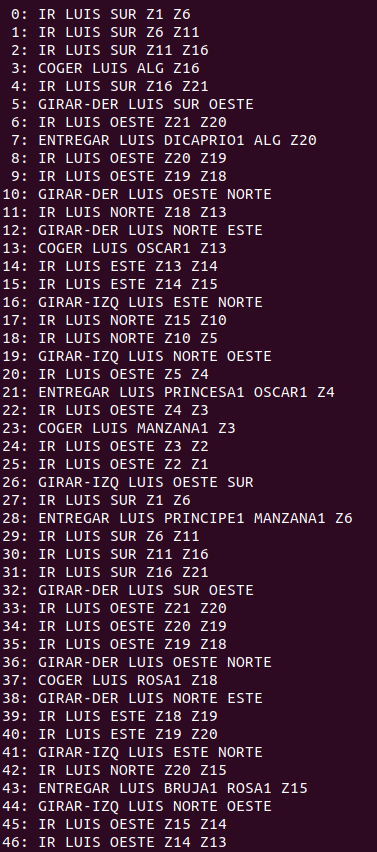
\includegraphics[width=\linewidth]{ej1-1.png}
		\caption{Primera parte de la ejecución}
		\label{fig:ej1-1}
	\end{minipage}
	\hspace{0.5cm}
	\begin{minipage}[b]{0.5\linewidth}
		\centering
		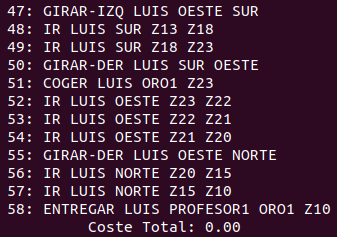
\includegraphics[width=\linewidth]{ej1-2.png}
		\caption{Fin del plan}
		\label{fig:ej1-2}
	\end{minipage}
\end{figure}

Como detalle, me gustaría explicar que para la posesión de objetos por parte de un Player utilizo dos predicados: posee ?x - Player ?o - objeto y mano-vacia ?x - Player. En el caso de COGER un objeto, una precondición es que tenga la mano vacía. Cuando lo coge, ya no tiene la mano vacía y además lo posee. Para dejar un objeto, la precondición es que lo posea y, tras dejarlo, ya no lo posee y tiene la mano vacía. Con esos dos predicados consigo minimizar las comprobaciones y darle un completo sentido al comportamiento.

\section{Ejercicio 2}

En el ejercicio 2 se añaden funciones: distancia entre zonas y distancia-total (recorrida por el Player). Una vez definidas las distancias entre zonas en el problema, la única modificación en el dominio sobre las acciones es en IR, donde cada vez que se consigue ir de una zona a otra se modifica la distancia-total añadiéndole la distancia entre la zona de partida y la de destino. El objetivo de este problema es que el Player reparta objetos entre todos los personajes recorriendo una distancia menor que una constante (a fijar por nosotros). Dicha constante determinará si el plan puede terminarse o no (una distancia demasiada corta haría imposible completar el recorrido). El resultado es el siguiente:


\begin{figure}[H]
	\begin{minipage}[b]{0.5\linewidth}
		\centering
		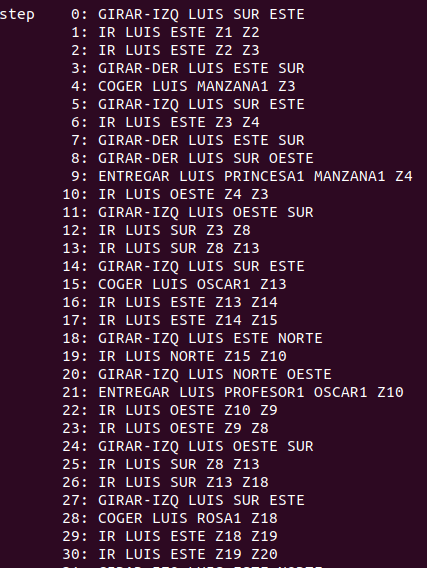
\includegraphics[width=\linewidth]{ej2-1.png}
		\caption{Primera parte del plan}
		\label{fig:ej2-1}
	\end{minipage}
	\hspace{0.5cm}
	\begin{minipage}[b]{0.5\linewidth}
		\centering
		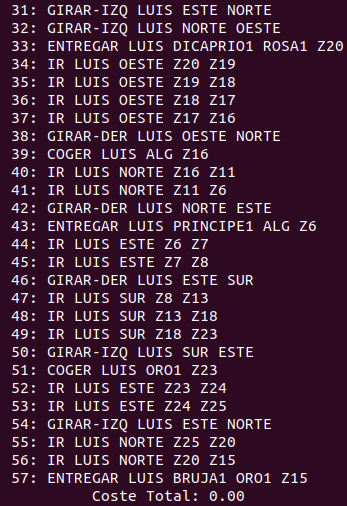
\includegraphics[width=\linewidth]{ej2-2.png}
		\caption{Fin del plan}
		\label{fig:ej2-2}
	\end{minipage}
\end{figure}

\section{Ejercicio 3}

En el ejercicio 3 se da un salto y el mundo se acerca más a Belkan. Ahora hay distintos tipos de zonas (bosque, agua, precipicio, arena y piedra) y nuevos objetos (zapatillas y bikini) de forma que solo se puede acceder al bosque si el Player tiene zapatillas y al agua si tiene bikini. Por supuesto, hay que añadir los objetos nuevos al catálogo y declaro una serie de predicados para identificar zonas y objetos (no se puede saber de qué tipo es un object en PDDL, por lo que hay que identificarlos con predicados). Son los siguientes:

\begin{itemize}
	\item (es-bikini ?o - objeto)
	\item (es-zapatilla ?o - objeto)
	\item (es-bosque ?z - zona)
	\item (es-agua ?z - zona)
	\item (es-precipicio ?z - zona)
	\item (es-arena ?z - zona)
	\item (es-piedra ?z - zona)
\end{itemize}

por tanto, cuando el Player quiere desplazarse a una zona, habrá que comprobar que no es un precipicio, si es bosque que tiene zapatillas y si es agua que tiene bikini. Además, COGER, DEJAR y ENTREGAR empiezan a tener en cuenta si el objeto era bikini o zapatillas para certificar que dejan de tenerlo o, por el contrario, empieza a poseerlo. \\

Otra modificación es que Player dispone de una mochila con un sólo un hueco de capacidad, de forma que surgen tres predicados nuevos (posee-mochila ?j - Player ?o -objeto, posee-mano ?j - Player ?o - objeto y mochila-vacia ?x - Player) y dos acciones nuevas: SACAR (teniendo la mano vacía y el objeto en la mochila) y METER (teniendo en la mano el objeto y la mochila vacía). \\ 

El resultado de este plan es más largo ya que hay zonas a priori que no puede atravesar y otras que nunca podrá (en el caso de precipicio). El objetivo sigue siendo el mismo; que todos los personajes tengan un objeto y se los entregue recorriendo una distancia menor que una constante: \\

\textbf{Nuevo mapa:}
\begin{center}
	\centering
	 ; z01  z2B  z03  z4A  z05 \\
	; z06  z7B  z08  z9A  z10 \\
	; z11 z12 z13 z14 z15 \\
	; z16 z17 z18B z19 z20 \\
	; z21P z22A z23A z24 z25A \\
\end{center}



\begin{figure}[H]
	\begin{minipage}[b]{0.5\linewidth}
		\centering
		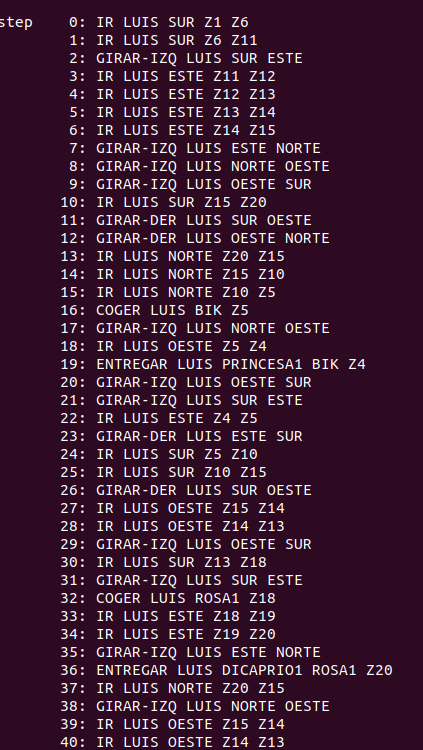
\includegraphics[width=\linewidth]{ej3-1.png}
		\caption{Primera parte del plan}
		\label{fig:ej3-1}
	\end{minipage}
	\hspace{0.5cm}
	\begin{minipage}[b]{0.5\linewidth}
		\centering
		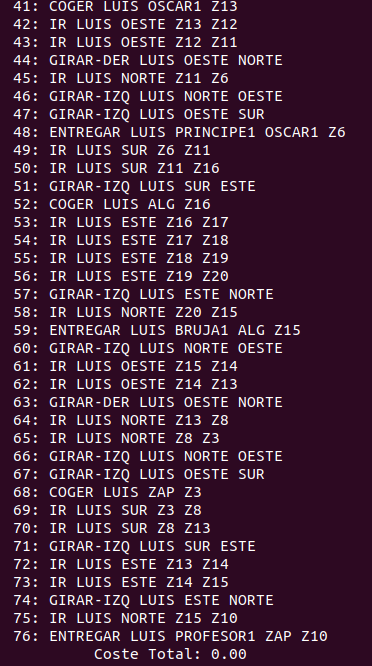
\includegraphics[width=\linewidth]{ej3-2.png}
		\caption{Fin del plan}
		\label{fig:ej3-2}
	\end{minipage}
\end{figure}

\section{Ejercicio 4}

Último ejercicio de la relación 1, en el que se propone contabilizar puntos en función de los objetos que Player entrega y los personajes que lo reciben. Para hacerlo de la forma más general posible, defino 10 constantes nuevas, 5 para identificar el tipo de personaje (tipoPersonaje) y 5 para identificar el tipo de objeto (tipoObjeto) y dos nuevos predicados (es-tipo-p y es-tipo-o). De esta manera, en el problema asigno a cada personaje y objeto su tipo y establezco que gana el jugador según los tipos de objetos y personajes a través de la función puntos. Además, acumulo los puntos que ha conseguido Player a través de la función puntos-jugador. A pesar de que parece algo sencillo, esto último se convierte en muy tedioso. Hay 5 tipos de objetos y de personajes, por tanto hay 25 combinaciones de ellos. En la función ENTREGAR se hace esa disquisición entre tipos para poder incrementar correctamente los puntos al jugador en función de los tipos.  \\

El resultado del plan, siendo los objetivos que todos los personajes reciban objeto, que la distancia recorrida sea menor que 500 y que el jugador acumule al menos 20 puntos, es el siguiente:


\begin{figure}[H]
	\begin{minipage}[b]{0.5\linewidth}
		\centering
		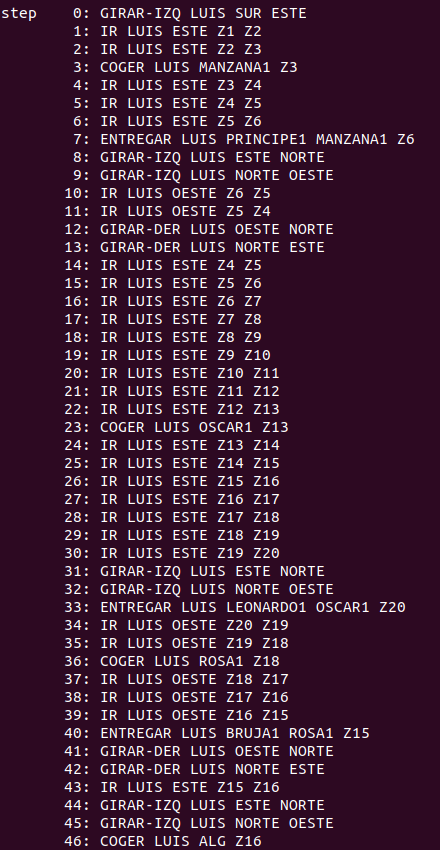
\includegraphics[width=\linewidth]{ej4-1.png}
		\caption{Primera parte del plan}
		\label{fig:ej4-1}
	\end{minipage}
	\hspace{0.5cm}
	\begin{minipage}[b]{0.5\linewidth}
		\centering
		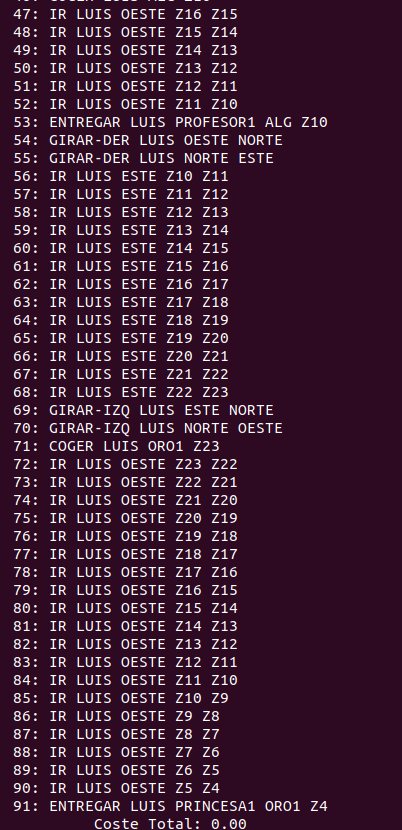
\includegraphics[width=\linewidth]{ej4-2.png}
		\caption{Fin del plan}
		\label{fig:ej4-2}
	\end{minipage}
\end{figure}

\section{Ejercicio 5}

La nueva relación empieza en el ejercicio 5 con el siguiente reto: cada personaje tiene un bolsillo mágico de longitud variable en el que almacenar cosas. Para afrontarlo, defino una nueva función llamada huecos-bolsillo ?p - personaje, de forma que en el init del problema definiré la cantidad de huecos libres que tiene cada personaje a priori. Con respecto a las acciones, las única modificación se encuentra en ENTREGAR, donde se añade una precondición que exija que el personaje tenga al menos un hueco en su bolsillo (>= (huecos-bolsillo ?p ) 1) y, una vez entregado el objeto, se decrementan los huecos disponibles (decrease (huecos-bolsillo ?p) 1). El resultado de la ejecución del plan, sabiendo que todos los personajes tienen un bolsillo con tres huecos, y exigiendo los mismos objetivos que en el ejercicio anterior es el siguiente:

\begin{figure}[H]
	\begin{minipage}[b]{0.5\linewidth}
		\centering
		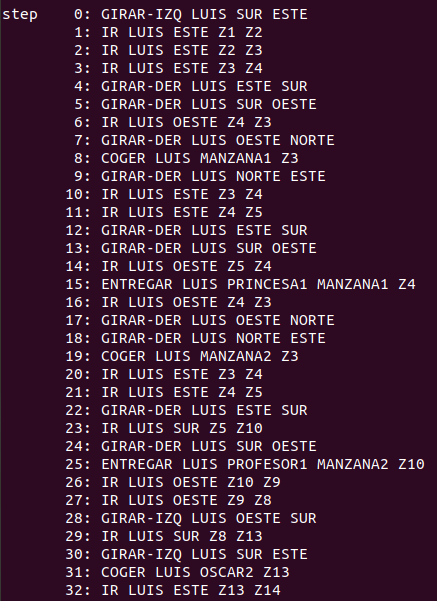
\includegraphics[width=\linewidth]{ej5-1.png}
		\caption{Primera parte del plan}
		\label{fig:ej5-1}
	\end{minipage}
	\hspace{0.5cm}
	\begin{minipage}[b]{0.5\linewidth}
		\centering
		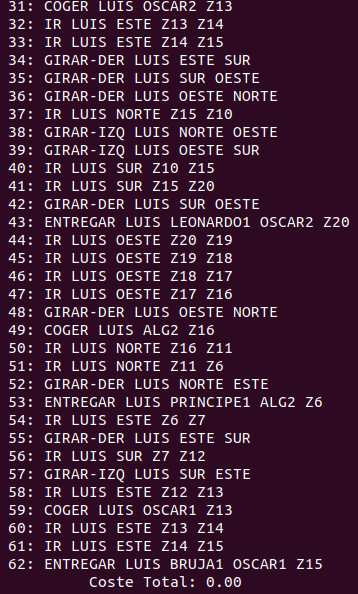
\includegraphics[width=\linewidth]{ej5-2.png}
		\caption{Fin del plan}
		\label{fig:ej5-2}
	\end{minipage}
\end{figure}

\section{Ejercicio 6}

Para conseguir que haya dos jugadores cooperantes, en los que cada uno consigue una puntuación mínima y entre los dos, una puntuación necesaria para superar el reto, es necesario definir dos nuevas funciones: puntos-indiv ?x - Player, que va contabilizando los puntos de un Player concreto y puntos-total (sustituye a puntos en el ejercicio anterior) que contabiliza la suma de los puntos-indiv de cada Player. Cuando se hace una entrega, en la parte que se discute qué tipoObjeto y tipoPersonaje son parte de la entrega, se incrementan tanto los puntos totales como los individuales con la cantidad que corresponda. En el problema, tras definir totalmente un Player extra con su posición, orientación, sus puntos a 0 y sus manos y mochila vacías, se requiere en el objetivo que cada uno tenga unos puntos mínimos y unos puntos totales. Téngase en cuenta que la función distancia es común, por lo que hay que subir el número de pasos para que el problema termine. Veamos la ejecución:

\begin{figure}[H]
	\begin{minipage}[b]{0.5\linewidth}
		\centering
		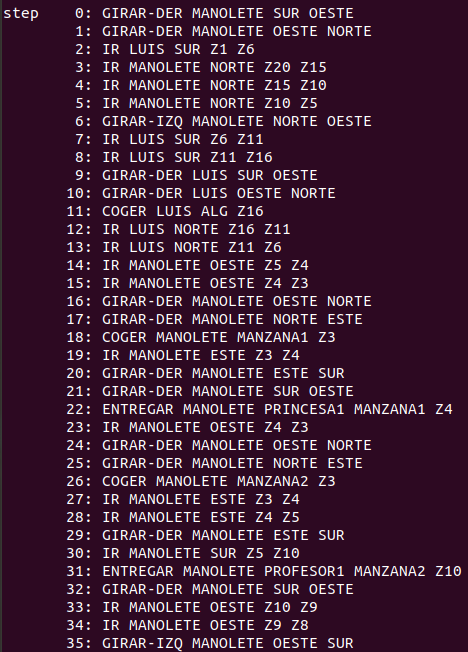
\includegraphics[width=\linewidth]{ej6-1.png}
		\caption{Primera parte del plan}
		\label{fig:ej6-1}
	\end{minipage}
	\hspace{0.5cm}
	\begin{minipage}[b]{0.5\linewidth}
		\centering
		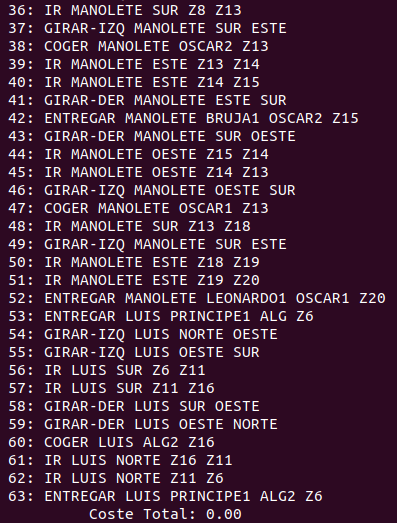
\includegraphics[width=\linewidth]{ej6-2.png}
		\caption{Fin del plan}
		\label{fig:ej6-2}
	\end{minipage}
\end{figure}

\section{Ejercicio 7}

Para resolver el ejercicio 7, en primer lugar es necesario definir dos tipos de Player: Picker y Dealer. Una vez hecho esto y gracias al diseño consistente que he ido haciendo, lo único que hace falta es refinar los argumentos en las acciones. Por ejemplo, a partir de ahora la acción COGER sólo la puede llevar a cabo un tipo Picker (antes era Player)y la función ENTREGAR-PERSONAJE (antes llamada ENTREGAR) sólo es efectuada por un Dealer. Se añade una nueva acción que se corresponde a la entrega de un objeto entre Picker y Dealer. DAR-DEALER, tras las comprobaciones necesarias (posesión y mano vacía, respectivamente) hace que el objeto pase al Dealer y el Picker no lo tenga. En el problema, como el Picker no va a entregar objetos, no necesita de una función que acumule sus puntos ni tiene sentido que añadamos un objetivo con tal fin. Por tanto, se reducen los objetivos a que todos los personajes tengan objetos, la distancia y la puntuación del Dealer.

\begin{figure}[H]
	\begin{minipage}[b]{0.5\linewidth}
		\centering
		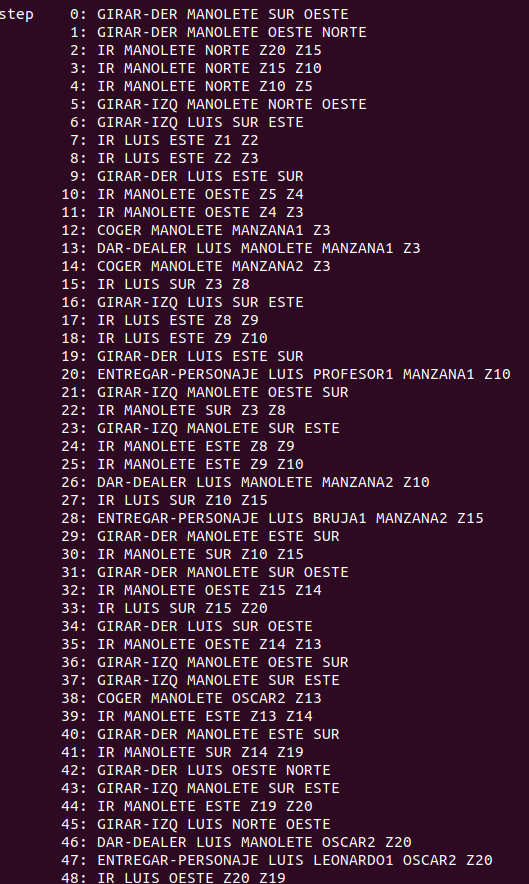
\includegraphics[width=\linewidth]{ej7-1.png}
		\caption{Primera parte del plan}
		\label{fig:ej7-1}
	\end{minipage}
	\hspace{0.5cm}
	\begin{minipage}[b]{0.5\linewidth}
		\centering
		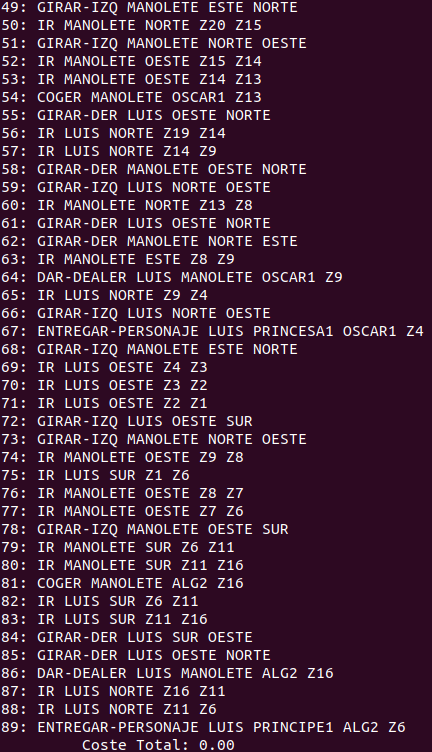
\includegraphics[width=\linewidth]{ej7-2.png}
		\caption{Fin del plan}
		\label{fig:ej7-2}
	\end{minipage}
\end{figure}

\end{document}
